\documentclass{article}
\usepackage[utf8]{inputenc}
\usepackage{fullpage} % Package to use full page
\usepackage{parskip} % Package to tweak paragraph skipping
\usepackage{amsmath}
\usepackage{hyperref}
\usepackage{cancel}
\usepackage{amssymb}
\usepackage{mathtools}
\usepackage{graphicx} % Required to insert images
\graphicspath{{./figs/}}
\usepackage{varwidth}
\usepackage{amstext}
\usepackage{amssymb}
%\usepackage{float}
\usepackage{array}
\usepackage[dvipsnames]{xcolor}
\usepackage{tikz} % Package for drawing
\usepackage{ctable}
\usepackage{tabu}
\usepackage{longtable}
\usepackage[section]{placeins}
\usepackage{natbib}
\usepackage{multirow}
\usepackage{subfigure}
\usepackage{caption}
\usepackage{verbatim}

\mathtoolsset{showonlyrefs=false}  %Makes it so only referenced equations are labeled 

\setcounter{secnumdepth}{0} %turn off section numbering

\title{The story of the dissipation correction}
\date{}

\newcommand\dsize[1]{\ensuremath{\mathcal{\scriptstyle {#1} } }} % dope new command for dissipation term
\newcommand\ensem[1]{\ensuremath{\left< {#1} \right>}} %ensemble average brakets
\newcommand\fpart[2]{\ensuremath{\frac{\partial {#1}}{\partial {#2} } }} % fractional style partial diff
\newcommand\avg[1]{\ensuremath{ \overline{{#1} }}}
\newcommand{\RN}[1]{%
  \textup{\uppercase\expandafter{\romannumeral#1}}%
}

\newcommand{\diss}{\dsize{E}}
\newcommand{\Deltait}{\mathit{\Delta}}

\makeatletter
\newcommand*\bigcdot{\mathpalette\bigcdot@{.5}}
\newcommand*\bigcdot@[2]{\mathbin{\vcenter{\hbox{\scalebox{#2}{$\m@th#1\bullet$}}}}}
\makeatother

\newenvironment{myeq}   %my totally awesome environment allowing for easy multiline math without too many labels
    {\begin{equation}
    \begin{gathered}
    }
    {
    \end{gathered}
    \end{equation}
    }
\begin{document}

\maketitle

\section{Synopsis}
Following the Xu.et al. paper the dissipation rate is modified to compensate for the limited resolution of the PIV. Second order structure functions are found along lines parallel to the shear layers, the value of the structure function in the inertial subrange is used used as the initial estimate of the dissipation rate. This estimate is then corrected to account for the resolution of the PIV. 

Due to the spacial averaging in the structure function method, the dissipation rate found this way is the average dissipation rate along the lines the structure function is defined. In order to have a 2D plane of dissipation rated averaged only through time a dissipation rate is estimated based on the fluctuating velocity gradients. This is then corrected based on the values obtained in the structure function method. 

\section{The works}

Second order structure functions are found along the lines parallel to the shear layers. The velocity component considered is the augmented v velocity, the $V_r$ matrix. The augmented flow field refers to the field transformed such that the lines parallel to the shear layers are the vertical axis. 

Structure functions are calculated to a maximum of $r = 15cm$ with equation \ref{StrucFunEq}. They are averaged along space and time. 

\begin{myeq}
    D_{LL}(r,t) = \ensem{(v(\xi + r ,t) - v(\xi,t))^2}
    \label{StrucFunEq}
\end{myeq}

In the limit of infinite Reynolds number the second order structure function will have the form $D_{LL} = C_2(\diss r)^{2/3}$ in the inertial subrange, with finite Reynolds number flows it's probably pretty close. If this assumption holds the derivative of the compensated structure function, \ref{CompStruct} will be 0 in the inertial subrange, and it's value will be the dissipation rate.  

\begin{myeq}
    \diss_{s_m} = \frac{1}{r}\left( \frac{D_{LL}(r)}{C_2} \right)^{3/2} \; \text{in inertial subrange}
    \label{CompStruct}
\end{myeq}

The dissipation rate from the structure functions is labeled $\diss_{s_m}$, the measured structure function dissipation rate. It is identified as the value of the compensated structure function at the location of the zero crossing of the first derivative of the compensated structure function, if the first derivative does not have a zero crossing, it is then identified as the zero crossing of the second derivative, representing an inflection in the compensated structure function. Structure functions, compensated structure functions and their derivatives are shown in figure \ref{StrucFun}, with the identified locations of the dissipation values marked as red circles.   

\begin{figure}[t]
    \centering
    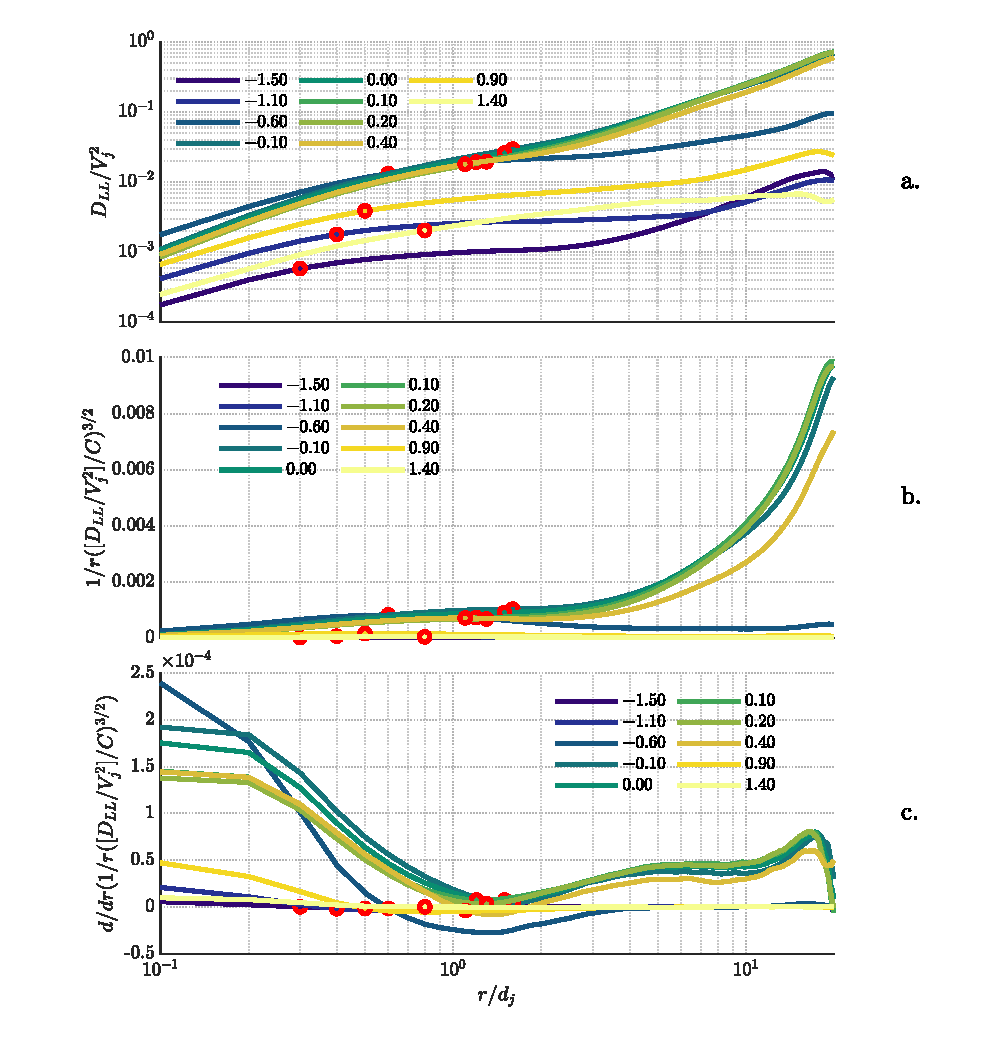
\includegraphics[scale = 0.75]{figs/PG_4Hz_StructureFuns.eps}
    \caption{a. Structure functions, b. Compensated structure functions, c. Derivative of compensated structure functions}
    \label{StrucFun}
\end{figure}

\begin{figure}[t]
    \centering
    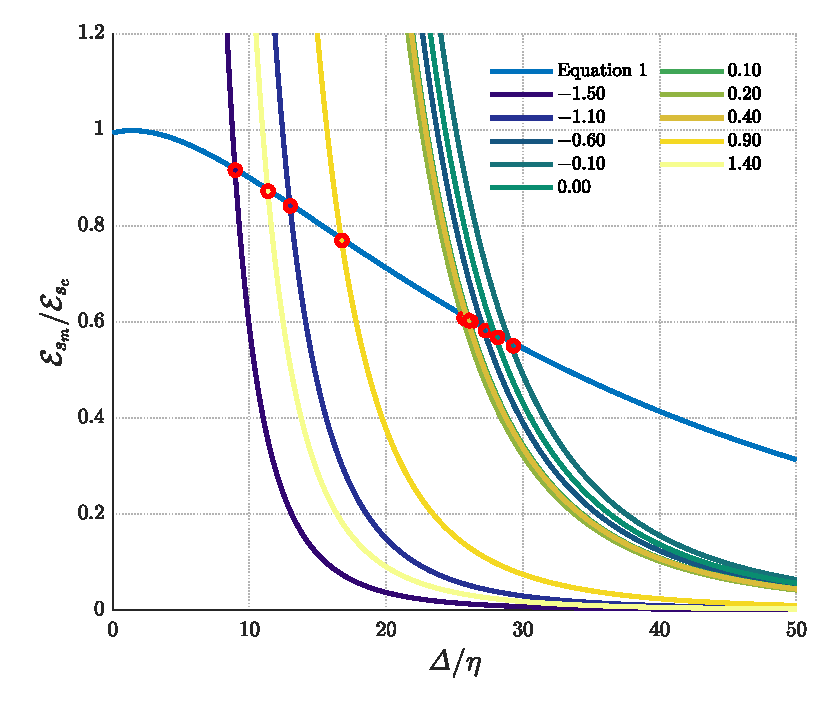
\includegraphics[scale = 0.6]{figs/Sdiff_Modification.eps}
    \caption{Structure function dissipatin modification}
    \label{SdiffMod}
\end{figure}

Due to the limited spatial resolution of the PIV velocity data the structure function method will under-predict the dissipation, the accuracy of the method increases as data resolution approaches $\eta$. An empirical model was developed with synthetic PIV data taken from a DNS data set. Solving the system of equations \ref{Correct1} and \ref{correct2} with known $\diss_{s_m}$, and data resolution, $\Deltait$ will yield $\diss_{s_c}$, the corrected structure function dissipation rate. Ya also get $\eta$, which is pretty cool but unnecessary.

\begin{myeq}
    \frac{\diss_{s_m}} {\diss_{s_c}} = \alpha_1 \exp{\left( \alpha_2 \frac{\Deltait}{\eta} \right)}
        + \beta_1 \exp{\left( \beta_2 \frac{\Deltait}{\eta} \right)}
    \label{Correct1}
\end{myeq}

\begin{myeq}
    \frac{\diss_{s_m}}{\diss_{s_c}} = \left( \frac{\diss_{D_{LL}} \Deltait^4 }{\nu^3} \right) \left(            \frac{\Deltait}{\eta} \right)^{-4} 
    \label{correct2}
\end{myeq}

\begin{figure}[b]
    \centering
    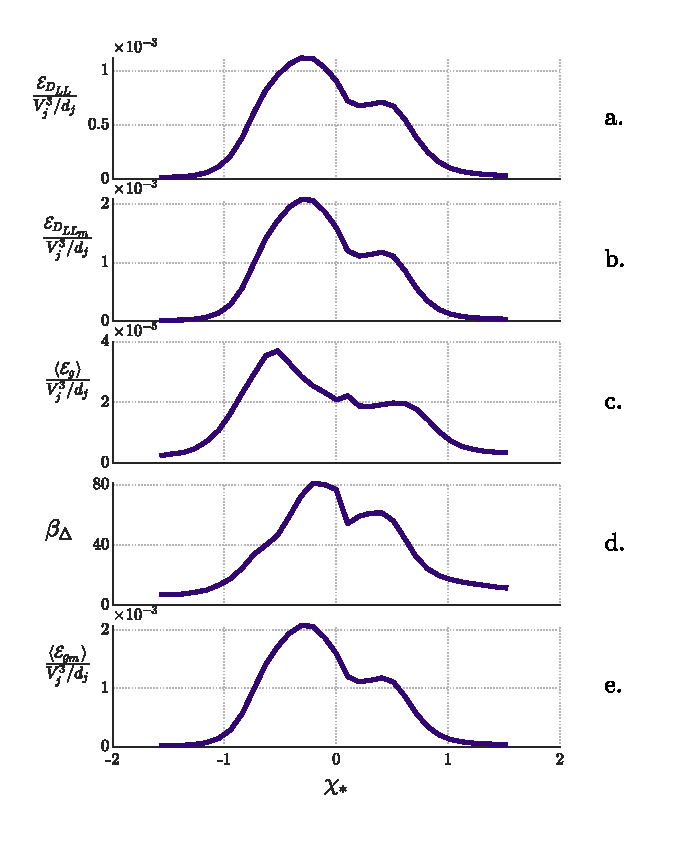
\includegraphics[scale = 0.75]{figs/PG_4Hz_Diss_Splots.eps}
    \caption{Export fig version}
    \label{DissPlot}
\end{figure}

This leaves us with one averaged dissipation value for every line along which the structure functions were calculated. In order to have values at every point in the flow the dissipation rate can be calculated with equation \ref{strainRate}. 

\begin{myeq}
    \diss = 2 \nu \ensem{S_{ij}S_{ij}}
    \label{strainRate}
\end{myeq}

However, we are limited in the directions in which we can take derivatives of the fluctuating velocities (or anything for that matter) in the PIV data. With an assumption of local isotropy equation \ref{strainRate} reduces to the form in equation \ref{localIso}, where only the in plane derivatives of the in place velocity components are required. 

\begin{myeq}
    \diss_{g_m} = \nu \left< 4\left( \fpart{u'_1}{x_1} \right)^2 + 4 \left( \fpart{u'_2}{x_2} \right)^2
        + 3 \left( \fpart{u'_1}{x_2} \right)^2 + 3 \left( \fpart{u'_2}{x_1} \right)^2 \right. \; \dots \\ 
        \left. + 4 \left( \fpart{u'_1}{x_1} \fpart{u'_2}{x_2} \right) + 6 \left( \fpart{u'_1}{x_2}
        \fpart{u'_2}{x_1} \right) \right>
    \label{localIso}
\end{myeq}

This calculation is also hampered by not being able to resolve the small scales in the PIV data. A corrected value of gradient dissipation, $\diss_{g_c}$ is related to the measured $\diss_{g_m}$ by a correction factor $\beta$,

\begin{myeq}
    \diss_{g_c}(x,y) = \beta_\Deltait \diss_{g_m}(x,y).
    \label{correctGrad}
\end{myeq}

The value of the correction factor $\beta$ is simply the ratio of corrected structure function dissipation, $\diss_{s_c}$ and the measured gradient dissipation, $\diss_{g_m}$ averaraged along the same direction as the structure functions are calculated and averaged, 

\begin{myeq}
    \beta_\Deltait = \frac{ \ensem{\diss_{s_c}} }{\ensem{\diss_{g_m}}}.
    \label{beta}
\end{myeq}


The measured, and corrected structure function dissipation rates, along with the mean of the measured gradient dissipation, the correction factor $\beta$, and the mean of the corrected gradient dissipation rates are all found in figure \ref{DissPlot}. Figure \ref{DissCont} shows the measured and corrected gradient dissipation rates as functions of $\xi_{*}$ and $\eta_{*}$.
%$\xi_*$ and $\r_*$. 






\begin{figure}
    \centering
    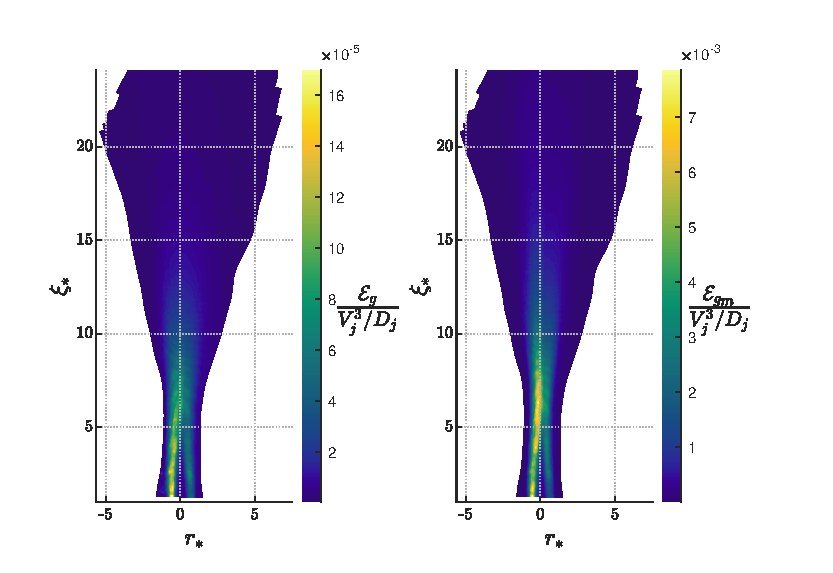
\includegraphics[]{figs/PG_4Hz_diss_contours.eps}
    \caption{Contours of the gradient calculated dissipation, and the corrected}
    \label{DissCont}
\end{figure}

\end{document}
